\documentclass[12pt,letterpaper]{article}
\usepackage[latin1]{inputenc}
\usepackage[spanish]{babel}
\usepackage{amsmath}
\usepackage{amsfonts}
\usepackage{amssymb}
\usepackage{graphicx}
\usepackage[hidelinks]{hyperref}
\usepackage{color}
\graphicspath{{Imagenes/}}
\usepackage[left=2cm,right=2cm,top=2cm,bottom=2cm]{geometry}
\author{M�rquez M�rquez Amairani Ivette}
\begin{document}
\begin{center}
\textbf{\huge{Universidad Politecnica de la Zona\\[0.5cm]Metropolitana de Guadalajara}}
\end{center}

\begin{center}

\includegraphics[width=0.65\textwidth]{Imagenes/UPCDLZMDG5783-logo.png}\\[0.2cm]
\end{center}
\vspace{0.5cm}
{\large\textbf{Evidencia:} 2.3 Explicar los arreglos y par�metros de los Amplificadores clase B\\[0.2cm]\textbf{Alumna:} M�rquez M�rquez Amairani Ivette\\[0.2cm]\textbf{Profesor:}Mor�n Garabito Carlos Enrique\\[0.2cm]\textbf{Carrera:}Ing.Mecatronica\\[0.2cm]\textbf{Grupo:} 4�B\\[0.2cm]\textbf{Fecha de entrega:} 08 de Octubre del 2019\\[02cm]}\\

\vspace{10cm}
\textbf{2.3 Explicar los arreglos y parametros de los Amplificadores clase B}\\[0.3cm]
Un Amplificador clase B nos manda una se�al de un semiciclo.
\begin{figure}[hbpt]
\centering
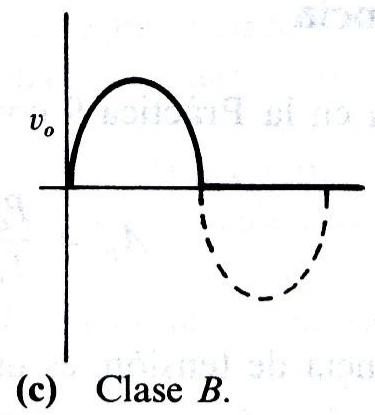
\includegraphics[width=8cm]{Imagenes/Captura_1.PNG}
\end{figure}

\vspace{0.3cm}

Un amplificador clase B amplifica un solo semiciclo de la se�al de entrada; esto implica situar el punto de trabajo en la region de corte, de tal forma, que s�lo al presentarse el semiciclo adecuado de  "Vi" el transistor pase a la regi�n activa. Cuando el semiciclo es el contrario, el transistor permanece en corte, al igual que en ausencia de se�al de entrada.\\ Si se quiere obtener una se�al de salida reflejo de la de entrada, se habran de disponer de forma adecuada, dos transistores, para que cada uno amplifique un semiciclo.\\
Los amplificadores clase B tienen rendimientos elevados, pero necesitan dos transistores para ofrecer una se�al de salida de forma igual a la de entrada.

\vspace{2cm}

{\large\textbf{Bibliograf�a}}\\
\begin{center}
\emph{Morales.V(2011).Amplificadores clase A y B - PDF.} Obtenido de:\\
\textcolor{blue}{https://electronicavm.files.wordpress.com/2011/03/amplificadores-clase-a-y-b1.pdf}\\[0.3cm]
\end{center}
 
\end{document}
